\chapter{Research Methodology} \label{chapter_four}

We will be using an IMU sensor for camera pose estimation to stabilize the video for this work. Based on the precision requirements of the pose-estimation algorithm we will be using a data-driven approach as classical signal processing and sensor fusion algorithms fail to provide this precision over a long period of time. For our data driven approach we build datasets using a camera and also simulation. To capture the video we are using a GoPro Hero 10 which provides synchronised image and sensor data capture. We also swapped the factory lens to a low Field of View (FOV) and high focal length lens. The simulation was build using Unreal Engine 4 and Microsoft AirSim. Table \ref{tab:technical_details} shows the technical specifications of the camera setup. For simulation similar camera parameters were used.

\begin{table}[ht]
    \centering
\begin{tabular}{ l| l | L }

     Image Sensor & 
     Sony & 
     Diagonal 7.85 mm (Type 1/2.3) 23.91 M CMOS Image Sensor with Square Pixel. \\
     \hline
     
     IMU Sensor & 
     Bosch & 
     6-axis IMU Sensor
     Accelerometer (A): 16-bit or 0.06 mg/LSB 
     Gyroscope (G): 16-bit or 0.004 dps/LSB  \\
     \hline
     
     Lens & 
     xx & 
     15° FOV and 00 mm focal length \\

\end{tabular}
    \caption{Technical Specification}
    \label{tab:technical_details}
\end{table}

\section{Data Collection}
Collecting data for any data driven approach is a challenging and an iterative process. The data or training data in this case are the readings coming from the IMU sensor and the target (ground truth) being the camera pose. Real data was collected by mounting the camera on a rig which had vibrations associated with it on movement. We made sure that the data depicts real life scenarios by moving the rig around in many different ways and let it vibrate and collect the data. The ground truth was generated using proprietary Zeiss software and is beyond the scope of this work. 

Then the data was collected from simulation based on the analysed real data and pushed beyond real data limits to account for even more challenging scenarios. Generating simulated data with accurate ground truth is a fast processes not requiring much post-processing. This also allowed us to tinker with noise and bias to make the neural network robust and generalize well.

\subsection{Data Analysis}
The data recorded from a camera-rig setup was analysed to find out the vibration and sensor parameters. Accelerometer variance was estimated to be $ 160 \mu g /\sqrt{Hz} $ and for gyroscope $ 0.008 dps /\sqrt{Hz}  $. 

% displacement data distribution table
\begin{table}[ht]
    \centering
\begin{tabular}{ c | L | L | L }
    
     Parameter  & 
     Mean ($ \mu $) & 
     Variance ($ \sigma^{2} $) &
     Standard Deviation ($ \sigma $)\\
     \hline
     
     $ A_{xy} $ & 
     $ 1.8944 mm $ & 
     $ 0.0018 mm^{2} $ &
     $ 1.3665 mm $ \\

      
     $ A_{z} $  & 
     $ 0.1135 mm $ & 
     $ 4.76e^{-6} mm^{2} $ &
     $ 0.0690 mm $ \\
     
     
     $ \omega_{xy} $ & 
     $ 3.6898 rad/s $ & 
     $ 5.9833 rad^{2}/s^{2} $ &
     $ 2.4460 rad/s $ \\
     
     
     $ \omega_{z} $& 
     $ 2.6835 rad/s $ & 
     $ 2.0765 rad^{2}/s^{2} $ &
     $ 1.0375 rad/s $ \\

     
     $ \tau_{xy} $ & 
     $ 2.5914 s $ & 
     $ 5.1898 s^{2} $ &
     $ 2.2781 s $ \\


     $ \tau_{z} $ & 
     $ 2.8396 s $ & 
     $ 5.8720 s^{2} $ &
     $ 2.4243 s $ \\

\end{tabular}
    \caption{Real Data displacement-vibration distributions}
    \label{tab:real_data_analysis_displacement}
\end{table}

% rotation data distribution table
\begin{table}[ht]
    \centering
\begin{tabular}{ c | L | L | L }

     Parameter  & 
     Mean ($ \mu $) & 
     Variance ($ \sigma^{2} $) &
     Standard Deviation ($ \sigma $)\\
     \hline
     
     $ \theta_{xy} $ & 
     $ 0.0094 rad $ & 
     $ 3.8729e^{-8} rad^{2} $ &
     $ 0.0062 rad $ \\

      
     $ \theta_{z} $  & 
     $ 0.0005 rad $ & 
     $ 6.0739e^{-8} rad^{2} $ &
     $ 0.0002 rad $ \\
     
     
     $ \omega_{xy} $ & 
     $ 3.8042 rad/s $ & 
     $ 6.3685 rad^{2}/s^{2} $ &
     $ 2.5236 rad/s $ \\

     
     $ \omega_{z} $& 
     $ 3.1763 rad/s $ & 
     $ 2.6238 rad^{2}/s^{2} $ &
     $ 1.6198 rad/s $ \\
   
     
     $ \tau_{xy} $ & 
     $ 2.6581 s $ & 
     $ 5.8362 s^{2} $ &
     $ 2.4158 s $ \\
    
     
     $ \tau_{z} $ & 
     $ 2.9316 s $ & 
     $ 4.7336 s^{2} $ &
     $ 2.1757 s $ \\

\end{tabular}
    \caption{Real Data rotational-vibration distributions}
    \label{tab:real_data_analysis_rotation}
\end{table}


%% Displacement distribution
\begin{figure}
    %%
    \begin{subfigure}{\linewidth}
    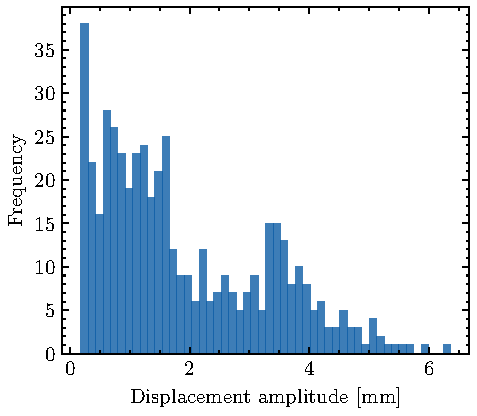
\includegraphics[width=.5\linewidth]{images/fig_chapter4/data_dist/1.pdf}\hfill
    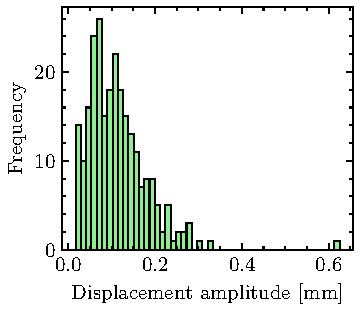
\includegraphics[width=.5\linewidth]{images/fig_chapter4/data_dist/2.pdf}
    \caption{Distribution of displacement amplitude $ A $ in XY(left) and Z(right) DoF [mm]}
    \end{subfigure}\par\medskip
    
    %%
    \begin{subfigure}{\linewidth}
    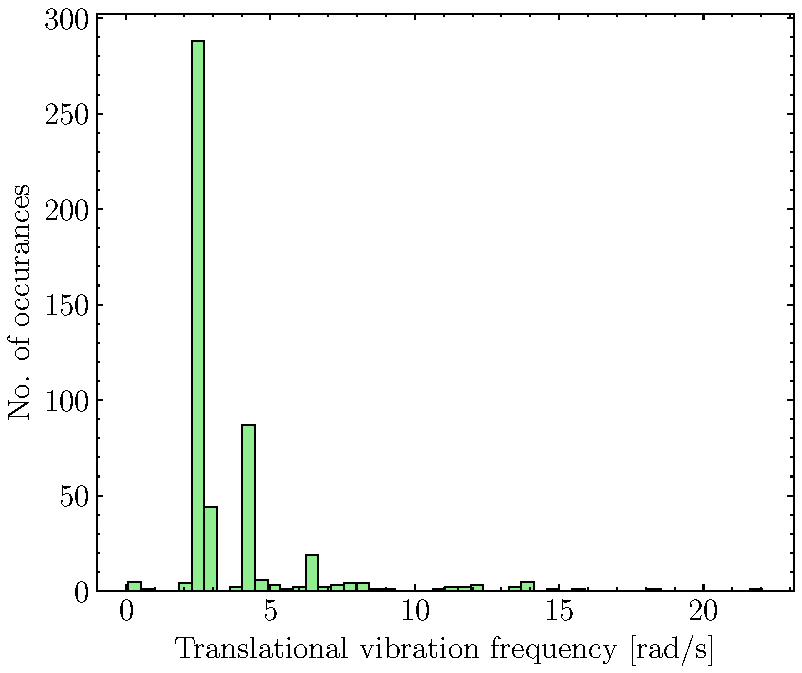
\includegraphics[width=.5\linewidth]{images/fig_chapter4/data_dist/3.pdf}\hfill
    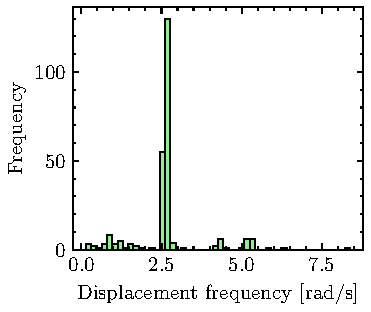
\includegraphics[width=.5\linewidth]{images/fig_chapter4/data_dist/4.pdf}
    \caption{Distribution of displacement frequency $ \omega $ in XY(left) and Z(right) DoF [mm]}
    \end{subfigure}\par\medskip
    
    %%
    \begin{subfigure}{\linewidth}
    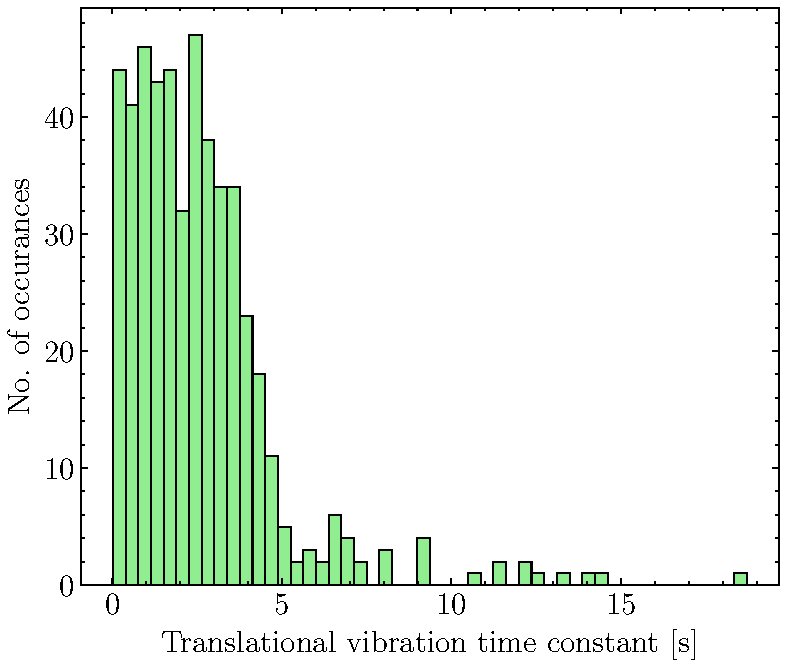
\includegraphics[width=.5\linewidth]{images/fig_chapter4/data_dist/5.pdf}\hfill
    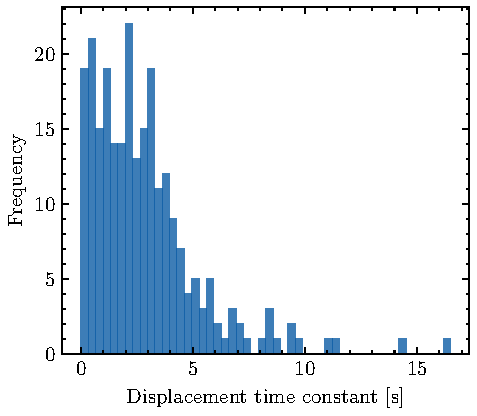
\includegraphics[width=.5\linewidth]{images/fig_chapter4/data_dist/6.pdf}
    \caption{Distribution of displacement time-constant $ \tau $ in XY(left) and Z(right) DoF [mm]}
    \end{subfigure}\par\medskip
\label{fig:data_distribution_disp}
\end{figure}

%% Rotation Distribution 
\begin{figure}
    %%
    \begin{subfigure}{\linewidth}
    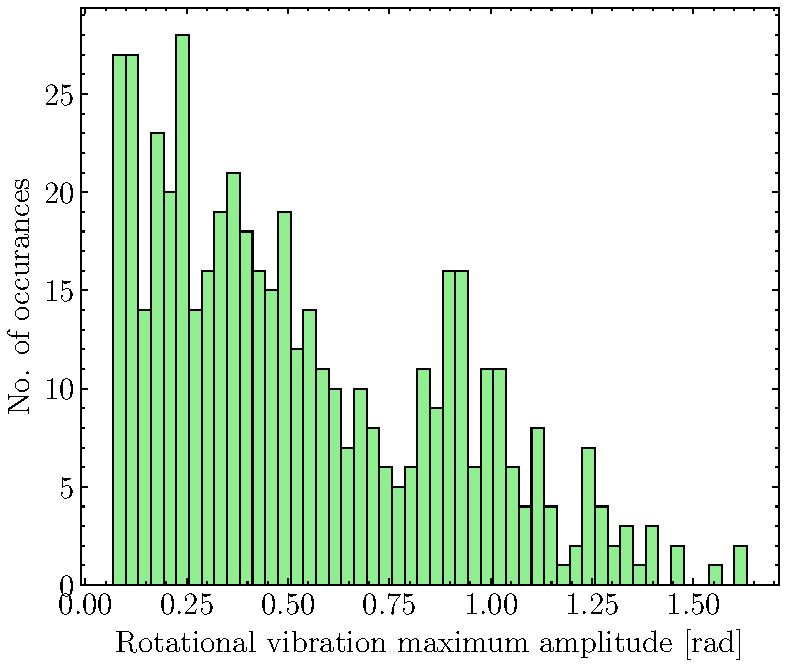
\includegraphics[width=.5\linewidth]{images/fig_chapter4/data_dist/7.pdf}\hfill
    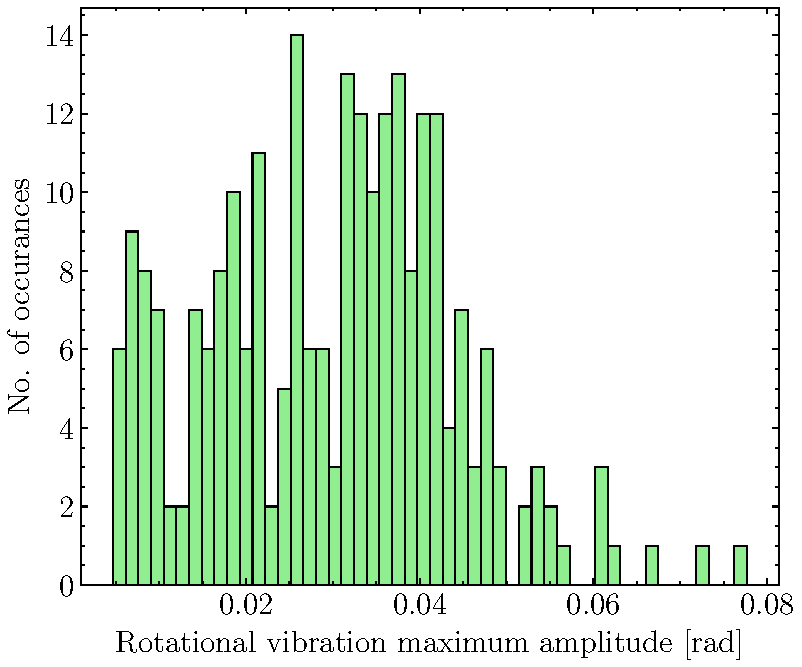
\includegraphics[width=.5\linewidth]{images/fig_chapter4/data_dist/8.pdf}
    \caption{Distribution of rotation amplitude $ \theta $ in XY(left) and Z(right) DoF [mm]}
    \end{subfigure}\par\medskip
    
    %%
    \begin{subfigure}{\linewidth}
    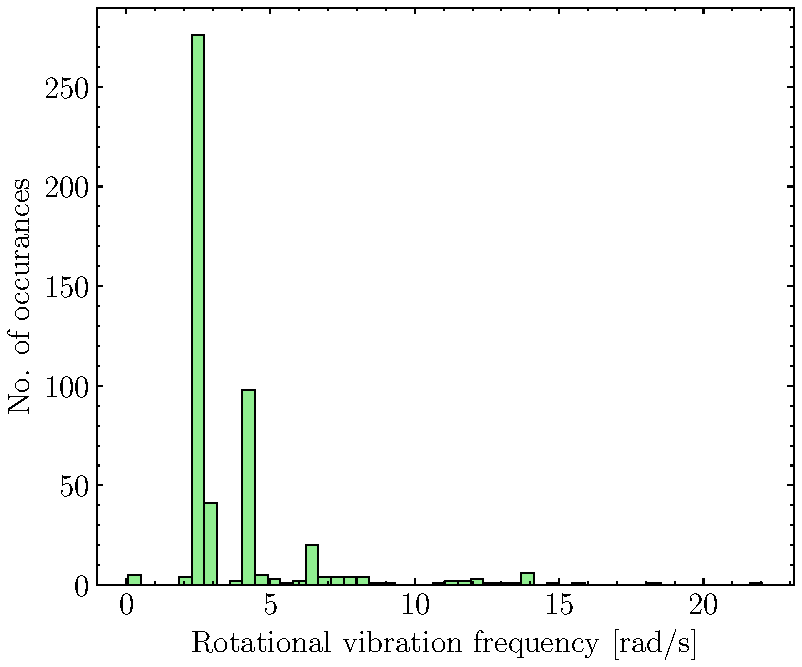
\includegraphics[width=.5\linewidth]{images/fig_chapter4/data_dist/9.pdf}\hfill
    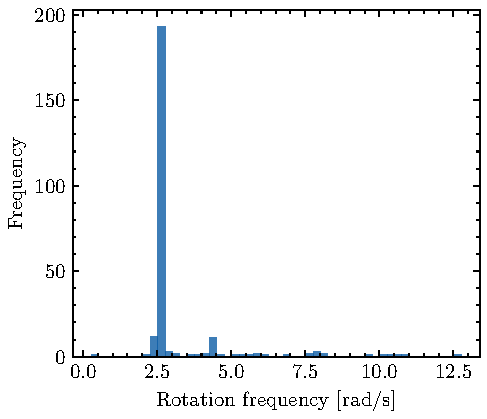
\includegraphics[width=.5\linewidth]{images/fig_chapter4/data_dist/10.pdf}
    \caption{Distribution of rotation frequency $ \omega $ in XY(left) and Z(right) DoF [mm]}
    \end{subfigure}\par\medskip
    
    %%
    \begin{subfigure}{\linewidth}
    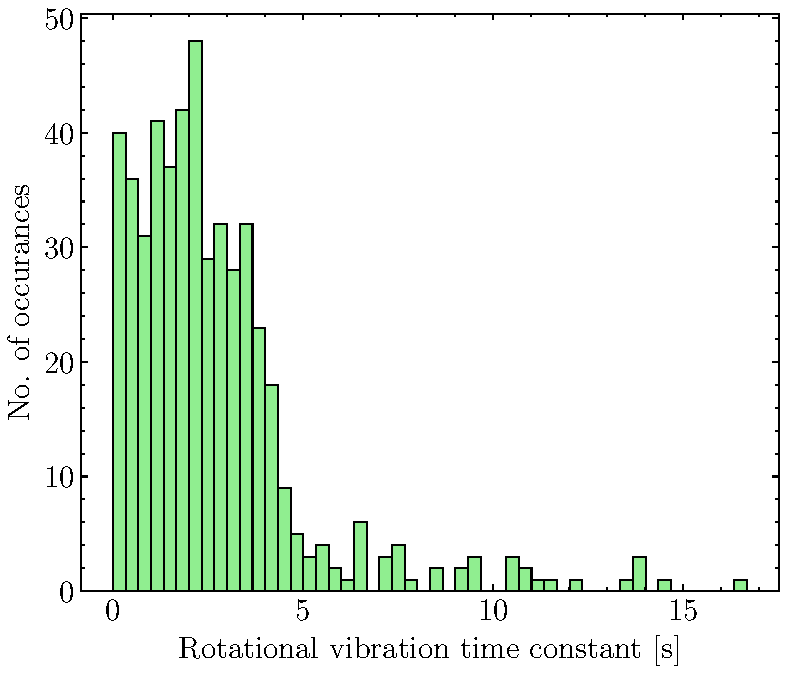
\includegraphics[width=.5\linewidth]{images/fig_chapter4/data_dist/11.pdf}\hfill
    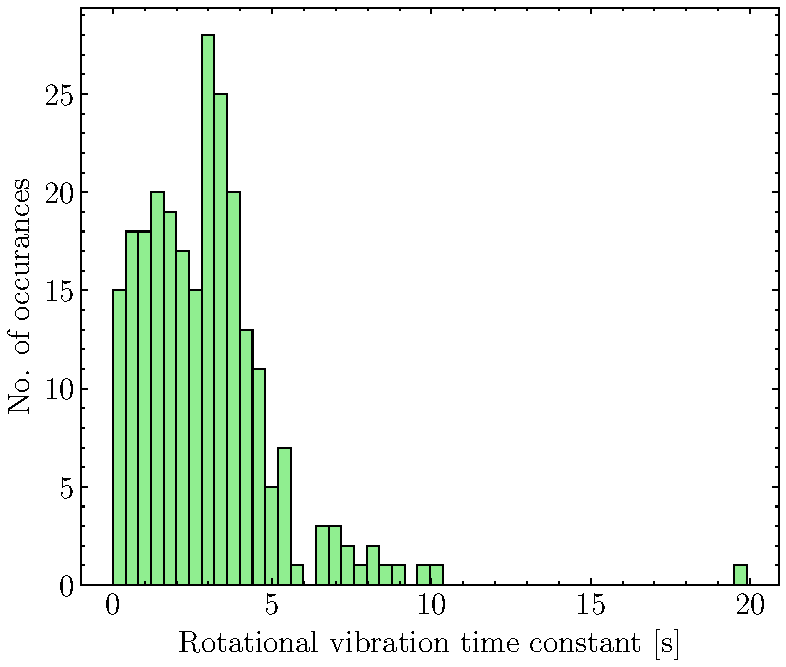
\includegraphics[width=.5\linewidth]{images/fig_chapter4/data_dist/12.pdf}
    \caption{Distribution of rotation time-constant $ \tau $ in XY(left) and Z(right) DoF [mm]}
    \end{subfigure}\par\medskip
\label{fig:data_distribution_rot}
\end{figure}

\begin{itemize}
\item Analyse Real Collected data to calculate Omega, Tow and Amplitude. 
\item Background of Dataset: How it was generated. 
\item What was the thought process. 
\item What kind of data we have.
\item Robustness of technique of Data Collection/Generation.
\end{itemize}



\section{Structuring of Data}
Data can be used in multiple ways. Explaining each way and why is it a good or a bad idea. What to put in networks. Sticking to realism.

\section{Mathematics for stabilisation}
Here we will see what exactly we are trying to find out: (R, T)

\section{Training and Testing of Various Neural Networks}
We will use various Neural Network types and Architectures.

\begin{itemize}
\item CNNs
\item RNNs: LSTMS 
\item Transformers
\item Temporal Fusion Transformers
\item CNNs
\item Resnets
\end{itemize}

\section{Image Stabilisation based on the Techniques Used}
We will see the Stabilized Videos and discuss about how they look visually to different people.


